\section{Исследовательский раздел}

% NOTE:
% Данный раздел содержит описание проведенных экспериментов и их результаты
% Должно быть обязательно указано, какую цель ставил перед собой автор работы при планировании экспериментов
% Какие предположения, гипотезы он надеялся подтвердить и опровергнуть и их помощью
% Результаты оформляются в виде графиков, диаграмм и/или таблиц
% (здесь также может быть проведено качественное и количественное сравнение с аналогами)

% Рек. Объем - 10-15 страниц

\subsection{Описание исследования}

% Исследовать временные характеристики и затраты памяти предложенного метода

\subsection*{Технические характеристики}

\subsection{Результаты исследования}

\subsection*{Вывод}

% В данном разделе будет проведено исследование времени работы алгоритма в зависимости от коэффициента увеличения документа при его преобразовании в изображение.
% С содержанием документа, на котором проводилось исследование, можно ознакомиться в приложении.
%
% \newpage
%
% \subsection{Постановка и условия исследования}
% % Высший класс — взять ту же idef0, которая была в первой главе, и изобразить зафиксированные и варьируемые факторы на ней, но не настаиваю. 
%
% На рисунке ниже приведена постановка задачи исследования, формализованная в виде IDEF0 диаграммы.
%
% \begin{figure}[H]
% 	\centering
% 	\includegraphics[width=\textwidth]{diag/varpar.pdf}
% 	\caption{Постановка задачи исследования}
% 	\label{fig:}
% \end{figure}
%
% \newpage
%
% \subsubsection*{Условия исследования}
%
% Технические характеристики устройства, на котором выполнялись замеры времени, представлены ниже.
% \begin{enumerate}
%     \item Процессор: \texttt{AMD Ryzen 7 4700U} 2.0 ГГц~\cite{amd}, 8 физических ядер, 8 потоков;
%     \item Оперативная память: 8 ГБ, \texttt{DDR4}, 3200 МГц;
%     \item Операционная система: \texttt{Arch}~\cite{arch};
%     \item Версия ядра: \texttt{6.14.6}.
% \end{enumerate}
%
% При выполнении замеров времени ноутбук был подключен к сети электропитания, был запущен браузер Chromium~\cite{chromium} с одной вкладкой, два терминала Alacritty~\cite{alacritty}, в которых были запущены веб-сервер приложения и Neovim~\cite{nvim} для фиксации получаемых данных.
%
% \subsection{Результаты исследования}
%
% В таблице ниже приведены результаты исследования.
% Данные в правой колонке являются усредненным значением из 10 замеров.
%
% \begin{table}[H]
% \centering
% \caption{Зависимость времени работы алгоритма от коэффициента увеличения документа при его преобразовании в изображение}
% % \begin{tabular}{|c|c|}
% % \begin{tabular}{|m{8cm}|m{8cm}|}
% \begin{tabular}{|m{6.85cm}|m{9.25cm}|}
% \hline
%     \,\hfill \textbf{Коэффициент увеличения} & \,\hfill \textbf{Среднее время разметки (с)} \hfill\, \\ \hline
%     \,\hfill 1 \hfill\, & \,\hfill 0.62 \hfill\, \\ \hline
%     \,\hfill 1.25 \hfill\, & \,\hfill 0.89 \hfill\, \\ \hline
%     \,\hfill 1.5 \hfill\, & \,\hfill 1.21 \hfill\, \\ \hline
%     \,\hfill 1.75 \hfill\, & \,\hfill 1.55 \hfill\, \\ \hline
%     \,\hfill 2 \hfill\, & \,\hfill 1.98 \hfill\, \\ \hline
%     \,\hfill 2.5 \hfill\, & \,\hfill 2.85 \hfill\, \\ \hline
%     \,\hfill 3 \hfill\, & \,\hfill 3.96 \hfill\, \\ \hline
%     \,\hfill 3.5 \hfill\, & \,\hfill 5.18 \hfill\, \\ \hline
%     \,\hfill 4 \hfill\, & \,\hfill 6.64 \hfill\, \\ \hline
%     \,\hfill 5 \hfill\, & \,\hfill 9.86 \hfill\, \\ \hline
%     \,\hfill 6 \hfill\, & \,\hfill 13.80 \hfill\, \\ \hline
%     \,\hfill 7 \hfill\, & \,\hfill 18.91 \hfill\, \\ \hline
%     \,\hfill 8 \hfill\, & \,\hfill 24.33 \hfill\, \\ \hline
%     \,\hfill 9 \hfill\, & \,\hfill 30.70 \hfill\, \\ \hline
%     \,\hfill 10 \hfill\, & \,\hfill 36.96 \hfill\, \\ \hline
% \end{tabular}
% \label{tab:}
% \end{table}
%
% Ниже табличные данные представлены графически.
%
% \begin{figure}[H]
% 	\centering
% 	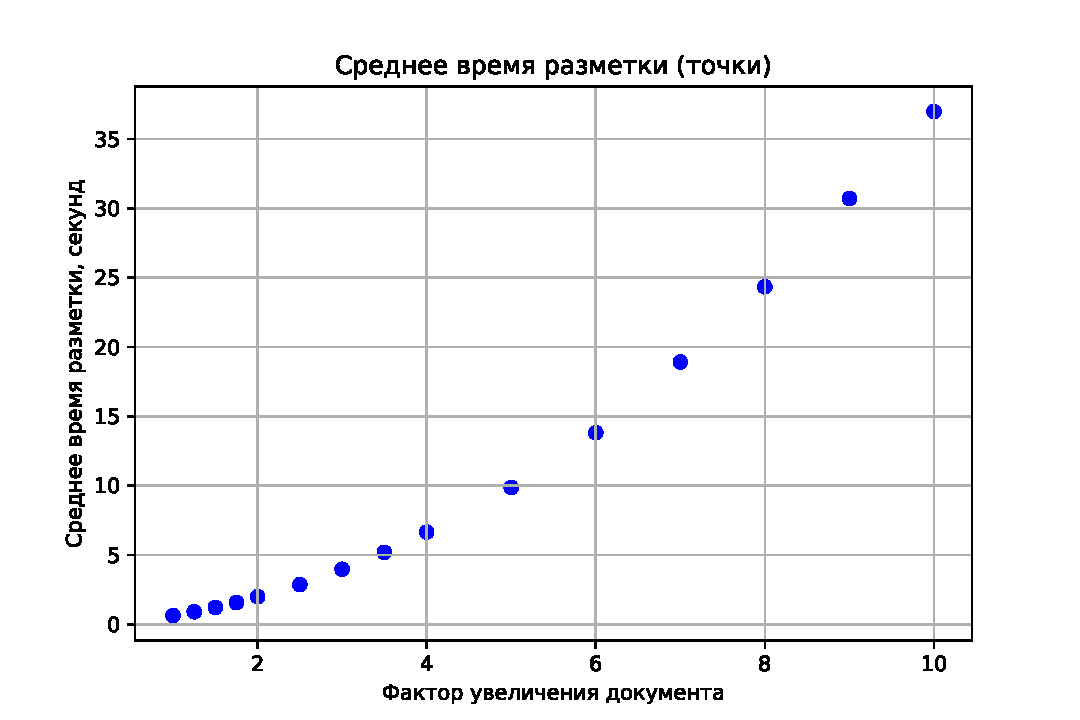
\includegraphics[width=\textwidth]{img/data.pdf}
% 	\caption{Зависимость времени работы алгоритма от коэффициента увеличения документа при его преобразовании в изображение, исходные данные}
% 	\label{fig:}
% \end{figure}
%
% Для определения зависимости времени разметки от фактора увеличения документа проведем степенную аппроксимацию на полученных данных.
%
% \begin{lstlisting}[caption={Степенная аппроксимация}]
% import numpy as np
% x = np.array([ ... ])
% y = np.array([ ... ])
% log_x = np.log(x)
% log_y = np.log(y)
% b, log_c = np.polyfit(log_x, log_y, 1)
% c = np.exp(log_c)
% print(f'y = {c:.3f} * x^{b:.3f}') # y = 0.583 * x^1.782
% \end{lstlisting}
%
% Таким образом, лучшей степенной аппроксимацией является уравнение $y = 0.583 \cdot x^{1.782}$, где $x$ --- фактор увеличения документа, а $y$ --- среднее время разметки.
% График данной аппроксимации в сравнении с исходными точками изображен на рисунке ниже.
%
% \begin{figure}[H]
% 	\centering
% 	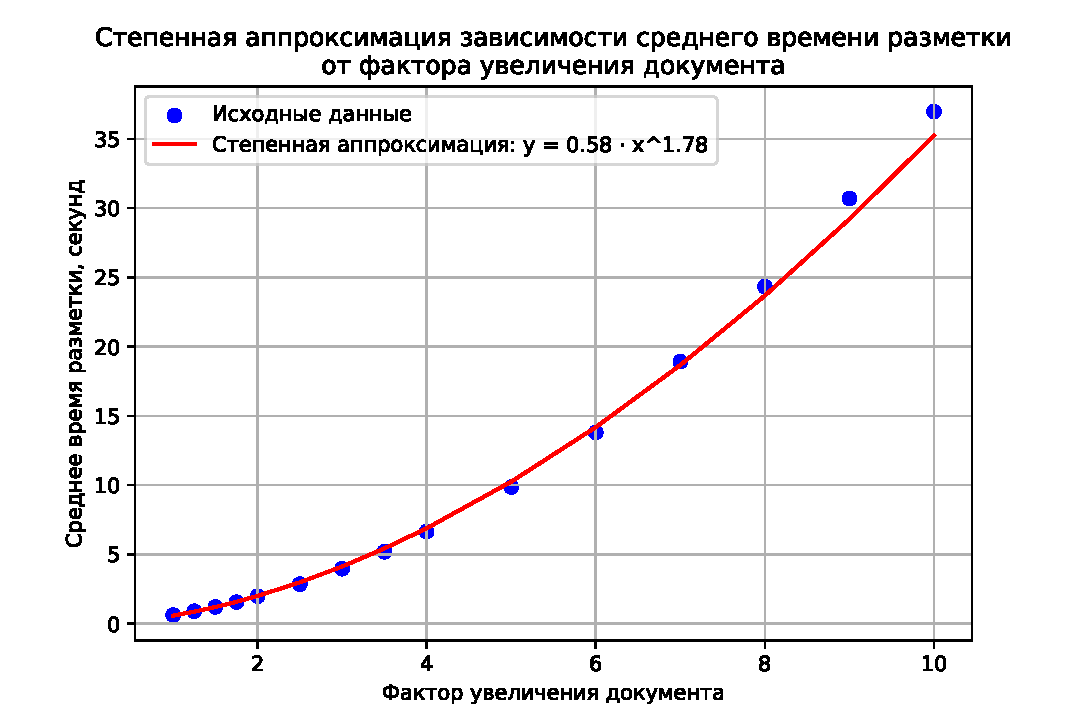
\includegraphics[width=\textwidth]{img/approx.pdf}
% 	\caption{Зависимость времени работы алгоритма от коэффициента увеличения документа при его преобразовании в изображение, степенная аппроксимация}
% 	\label{fig:}
% \end{figure}
%
% \subsection*{Вывод}
%
% В ходе проведенного исследования выяснилось, что наилучшей степенной аппроксимацией зависимости времени разметки от фактора увеличения документа при его преобразовании в изображение является уравнение $y = 0.583 \cdot x^{1.782}$, где $x$ --- фактор увеличения документа, а $y$ --- среднее время разметки.
%
